\begin{figure}
\begin{fullpage}
        \begin{center}
        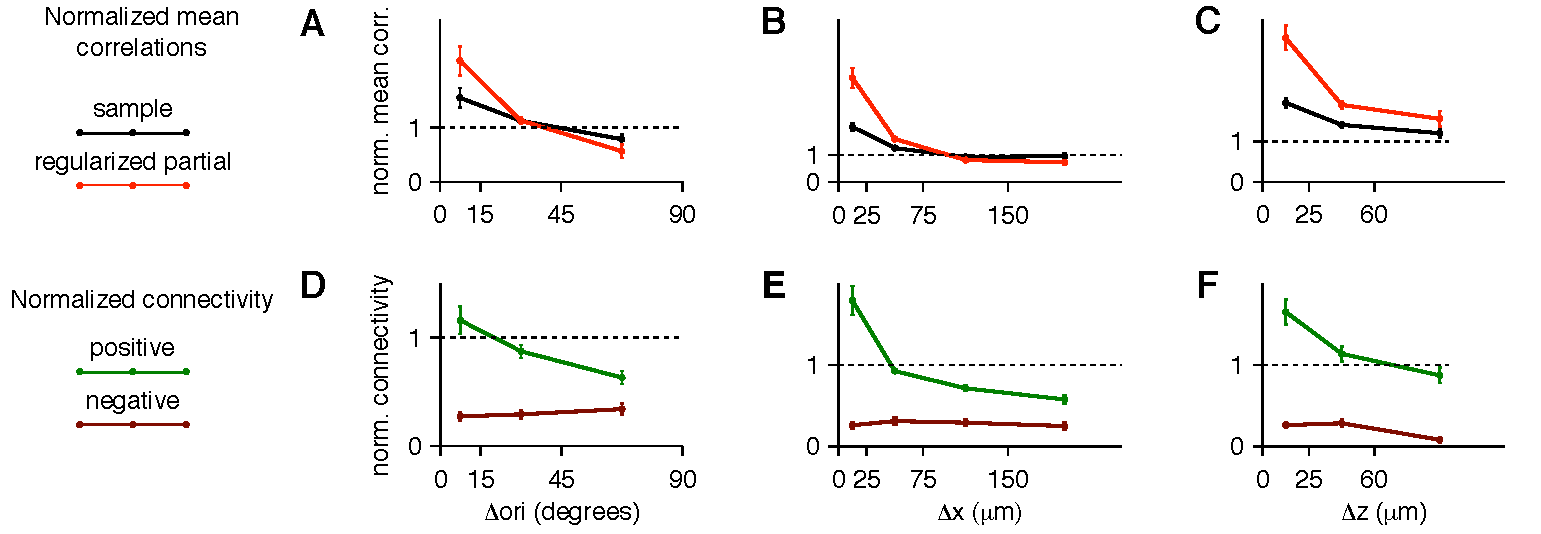
\includegraphics[width=\textwidth]{./figures/OrientationAndDistance.pdf}
        \end{center}
\caption[Relationship between functional connectivity and circuit architecture]{
{\bf Relationship between functional connectivity and circuit architecture.} 
The error bars mark the standard errors of the means. Five sites with highest connectivity (see Fig.~\ref{fig:5} B) were selected for this analysis.
{\bf A--C.} Normalized mean sample correlations (black) and normalized mean partial correlations (red) estimated by $C_{\sf sparse+latent}$ across $n=5$ imaged sites. The values in each bin are normalized by the means across the entire site, shown in Fig.~\ref{fig:5} C, to make the effects more comparable across the sites.
{\bf A.} Mean partial correlations in $C_{\sf sparse+latent}$ depend on $\Delta ori$ more strongly than mean sample correlations.
{\bf B.} Mean partial correlations in $C_{\sf sparse+latent}$ depend on $\Delta x$ more strongly than mean sample correlations. Only horizontally aligned cell pairs with $\Delta z<30\,\mu m$ were considered.
{\bf C.} Mean partial correlations in $C_{\sf sparse+latent}$ depend on $\Delta z$ more strongly than mean sample correlations. Only vertically aligned cell pairs with $\Delta x<30\,\mu m$ were considered.    {\bf D--F.} Normalized positive connectivity (green) and normalized negative connectivity (dark red) inferred by the $C_{\sf sparse+latent}$ estimator in $n=5$ imaged sites.
Here ``connectivity'' refers to the fraction of the non-zero elements in the sparse component $S$ of the $C_{\sf sparse+latent}$ estimator, which describes inferred direct interactions between specific pairs of the recorded neurons. Positive and negative connectivities refer to the fractions of the positive and negative partial correlations computed from  $S$, respectively.  ``Normalized positive connectivity'' is the ratio of the positive connectivity for pairs meeting a given condition, \emph{e.g.}~similar tuning with $\Delta ori <15^{\circ}$, to the average connectivity over the entire site.  Normalized negative connectivity is computed similarly for the negative connectivity.  The average connectivity across sites is shown in Fig.~\ref{fig:5} B with only the five most connected sites included in the analysis.  The normalization made the effects of tuning and distance more comparable across sites.
{\bf D.} Positive connectivity decreases with $\Delta ori$ whereas negative connectivity does not.
{\bf E.} Positive connectivity decays with $\Delta x$ whereas negative connectivity does not, within the examined range.
{\bf F.} Positive connectivity decays with $\Delta z$. Negative connectivity does not decay for small values of $\Delta z$.

}\label{fig:6}

\end{fullpage}
\end{figure}
